
As mentioned by Samothrakis \cite{Samothrakis2005}, the subject of gravity currents has examples of transport phenomena in the atmosphere and the ocean, snow avalanches, pyroclastic flows, and the sudden release of a dense gas resulted from the containment tank failure.

The numerical simulations of gravity currents have a similar setup to the experiment of gravity current propagation into a linearly stratified fluid demonstrated by Maxworthy et al. \cite{Maxworthy02}. A fixed volume of fluid with higher salinity at the left boundary of a tank is released into the ambient fluid with salinity linearly stratified. The tank is $1.4 \ m$ long, $0.2 \ m$ wide, and $0.3 \ m$ deep. The bottom slope is zero. The water depth is $0.15 \ m$.

%and the salinity diffusivity is $10^{-5} \ m^2/s$.

\begin{comment}
The numerical model uses uniform grid spacings of $0.01 \ m$ in $x$, $0.04 \ m$ in $y$, and $0.0025 \ m$ in $z$. The time step ranges from $0.05 \ sec$ to $0.001 \ sec$. The diffusion coefficient of velocity is tested from $10^{-4} \ m^2/s$ to $10^{-6} \ m^2/s)$.
\end{comment}

The density of the fluid is estimated from the simplified equation of state \cite{Gill1982},
\begin{equation}
\rho = \rho_o +0.75887 \ s
\end{equation}
where the salinity $s$ is the mass of salt in gram dissolved per thousand gram seawater. The temperature is assumed to be constant and is equal to $20^o C$. The pressure is set to $1 \ atmosphere$. The salinity in the fixed volume to be released in the left tank is tested from $135$ to $155 \ g/1000g$. The maximum salinity in the linearly stratified environment fluid is tested from $40$ to $80 \ g/1000g$. The viscosity is set to $10^{-6} \ m^2/s$. The diffusivity of salinity is tested from $10^{-4} \ m^2/s$ to $10^{-6} \ m^2/s$.


The fitting curve equation proposed by Maxworthy et. al. \cite{Maxworthy02} is:
\be
Fr=C+K \cdot log_{10}R
\label{eqn:gravitycurrent-fitting}
\ee
\be
C=a+b \cdot log_{10}(h/H), \ K=c+d \cdot log_{10}(h/H)
\ee
\be
a=0.270, \ b=0.246, \ c=0.935, \ d=0.307
\ee
where $h$ is the depth of the fixed-volume denser fluid and the froude number $Fr$ is defined as:
\be
Fr=\f{V_o}{NH}
\ee
\be
N^2=\f{g}{\rho_o} (-\f{d\rho}{dz})
\ee
\be
\f{d\rho}{dz}=\f{\rho_o-\rho_b}{H}
\ee
where $V_o$ is the initial velocity of the gravity current front. In the numerical simulation, this initial velocity $V_o$ is computed from the front location at $t=6 \ sec$. $H$ is the water depth. $N$ is the intrinsic frequency.

The parameter $R$ is the ratio of the effective density difference and the stratification density difference:
\be
R=\f{\rho_c-\rho_o}{\rho_b-\rho_o}
\ee
where $\rho_o$ is the smallest density at the top of the fluid, $\rho_b$ is the largest density of the ambient fluid at the bottom, and $\rho_c$ is the density of the fixed-volume denser fluid to be released.

The initial numerical test uses three different grid resolutions to simulate the Figure 9 case (Fig \ref{fig:Maxworthy02JFM}).
\be
h/H=2/3, Fr=0.489, N=1.981s^{-1}, H=15cm
\ee
\be
Fr=0.2267+0.881 log \ R
\ee
\be
N^2= \f{g(\rho_b-\rho_o)}{H\rho_o}
\ee
From the above equations and the assumption of $\rho_o=1008$, the other two densities can be calculated as $\rho_b=1068.55(g/cm^3)$,  $\rho_c=1128.19(g/cm^3)$ ($S_b=79.79$, $S_c=158.38$); and the initial velocity is $v_o = 0.1453(m/s)$. Therefore the maximum distance the gravity current travels in 6.3(sec) is $0.1453 \times 6.3 \sim 0.915(m)$, and the distance from the left wall is $0.915 + 0.2 \sim 1.115(m)$. The uniform grid spacings are from $0.04 \ m$ to $0.01 \ m$ in the horizontal direction and from $0.005 \ m$ to $0.0025 \ m$ in the vertical direction. For the low resolution case (Fig \ref{fig:GraCur-1-Dom-Low-RCIP1-Slip}), $\Delta x = 0.04 \ m$, $\Delta z= 0.005 \ m$, $\Delta t= 0.009 \ sec$.
For the medium resolution (Fig \ref{fig:GraCur-1-Dom-Medium-RCIP1-Slip}), $\Delta x = 0.02 \ m$, $\Delta z= 0.005 \ m$, $\Delta t = 0.009 \ sec$. For the high resolution (Fig \ref{fig:GraCur-1-Dom-High-RCIP1-Nslip}), $\Delta x= 0.01 \ m$, $\Delta z= 0.0025 \ m$, $\Delta t= 0.0018 \ sec$.

If the velocity of the gravity current is around $0.1 (m/s)$, then the Reynolds number can be approximated with the kinematic viscosity of water $\nu \sim 10^{-6} (m^2/s)$ and the water depth $l=0.15 (m)$,
\be
Re \sim \f{0.1 \times 0.15}{10^{-6}}= 15000
\ee
If the smallest Kolmogorov's length scale $\eta$ is to be resolved in the numerical model \cite{Tennekes1972},
\be
Re_{\Delta x}=Re_{\eta} = u \eta/ \nu=1
\ee
then the number of grids in one dimension will be
\be
N= l/\eta = Re^{3/4}_l \sim 10^6 %3.7 \times 10^6
\ee
and the grid size will be the order of $10^{-5} (m)$. However, the purpose of this simulation is not focusing on the brute force of the direct numerical simulation, but rather a preliminary test for the later experiments with the adjustable non-hydrostatic method in Chapter \ref{chapter:ANH} and the receding boundary method in Chapter \ref{chapter:RBM}. Therefore a qualitative convergence test will be performed with different resolutions with the staggered grid in Section \ref{chapter:NumericalTest-Staggered} and with the colocated grid in Section \ref{chapter:NumericalTest-colocated}.

\begin{figure}[htbp]
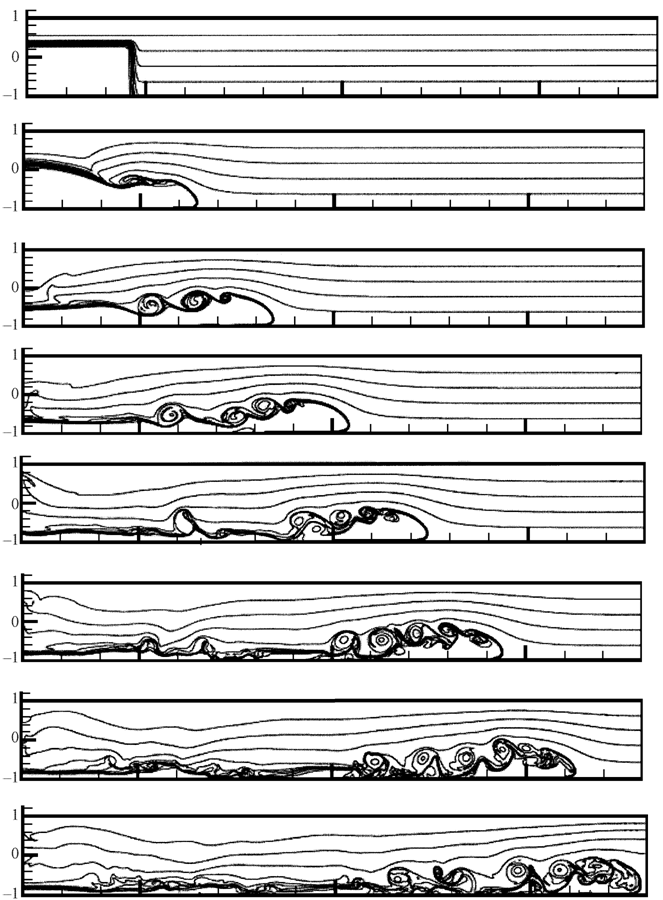
\includegraphics[width=5.5in]{../figures/GraCur/Maxworthy02JFM.pdf}
\caption{Sketch of gravity current experiment Fig 9 case from \cite{Maxworthy02}.}
\label{fig:Maxworthy02JFM}
\end{figure}

\begin{figure}[htbp]
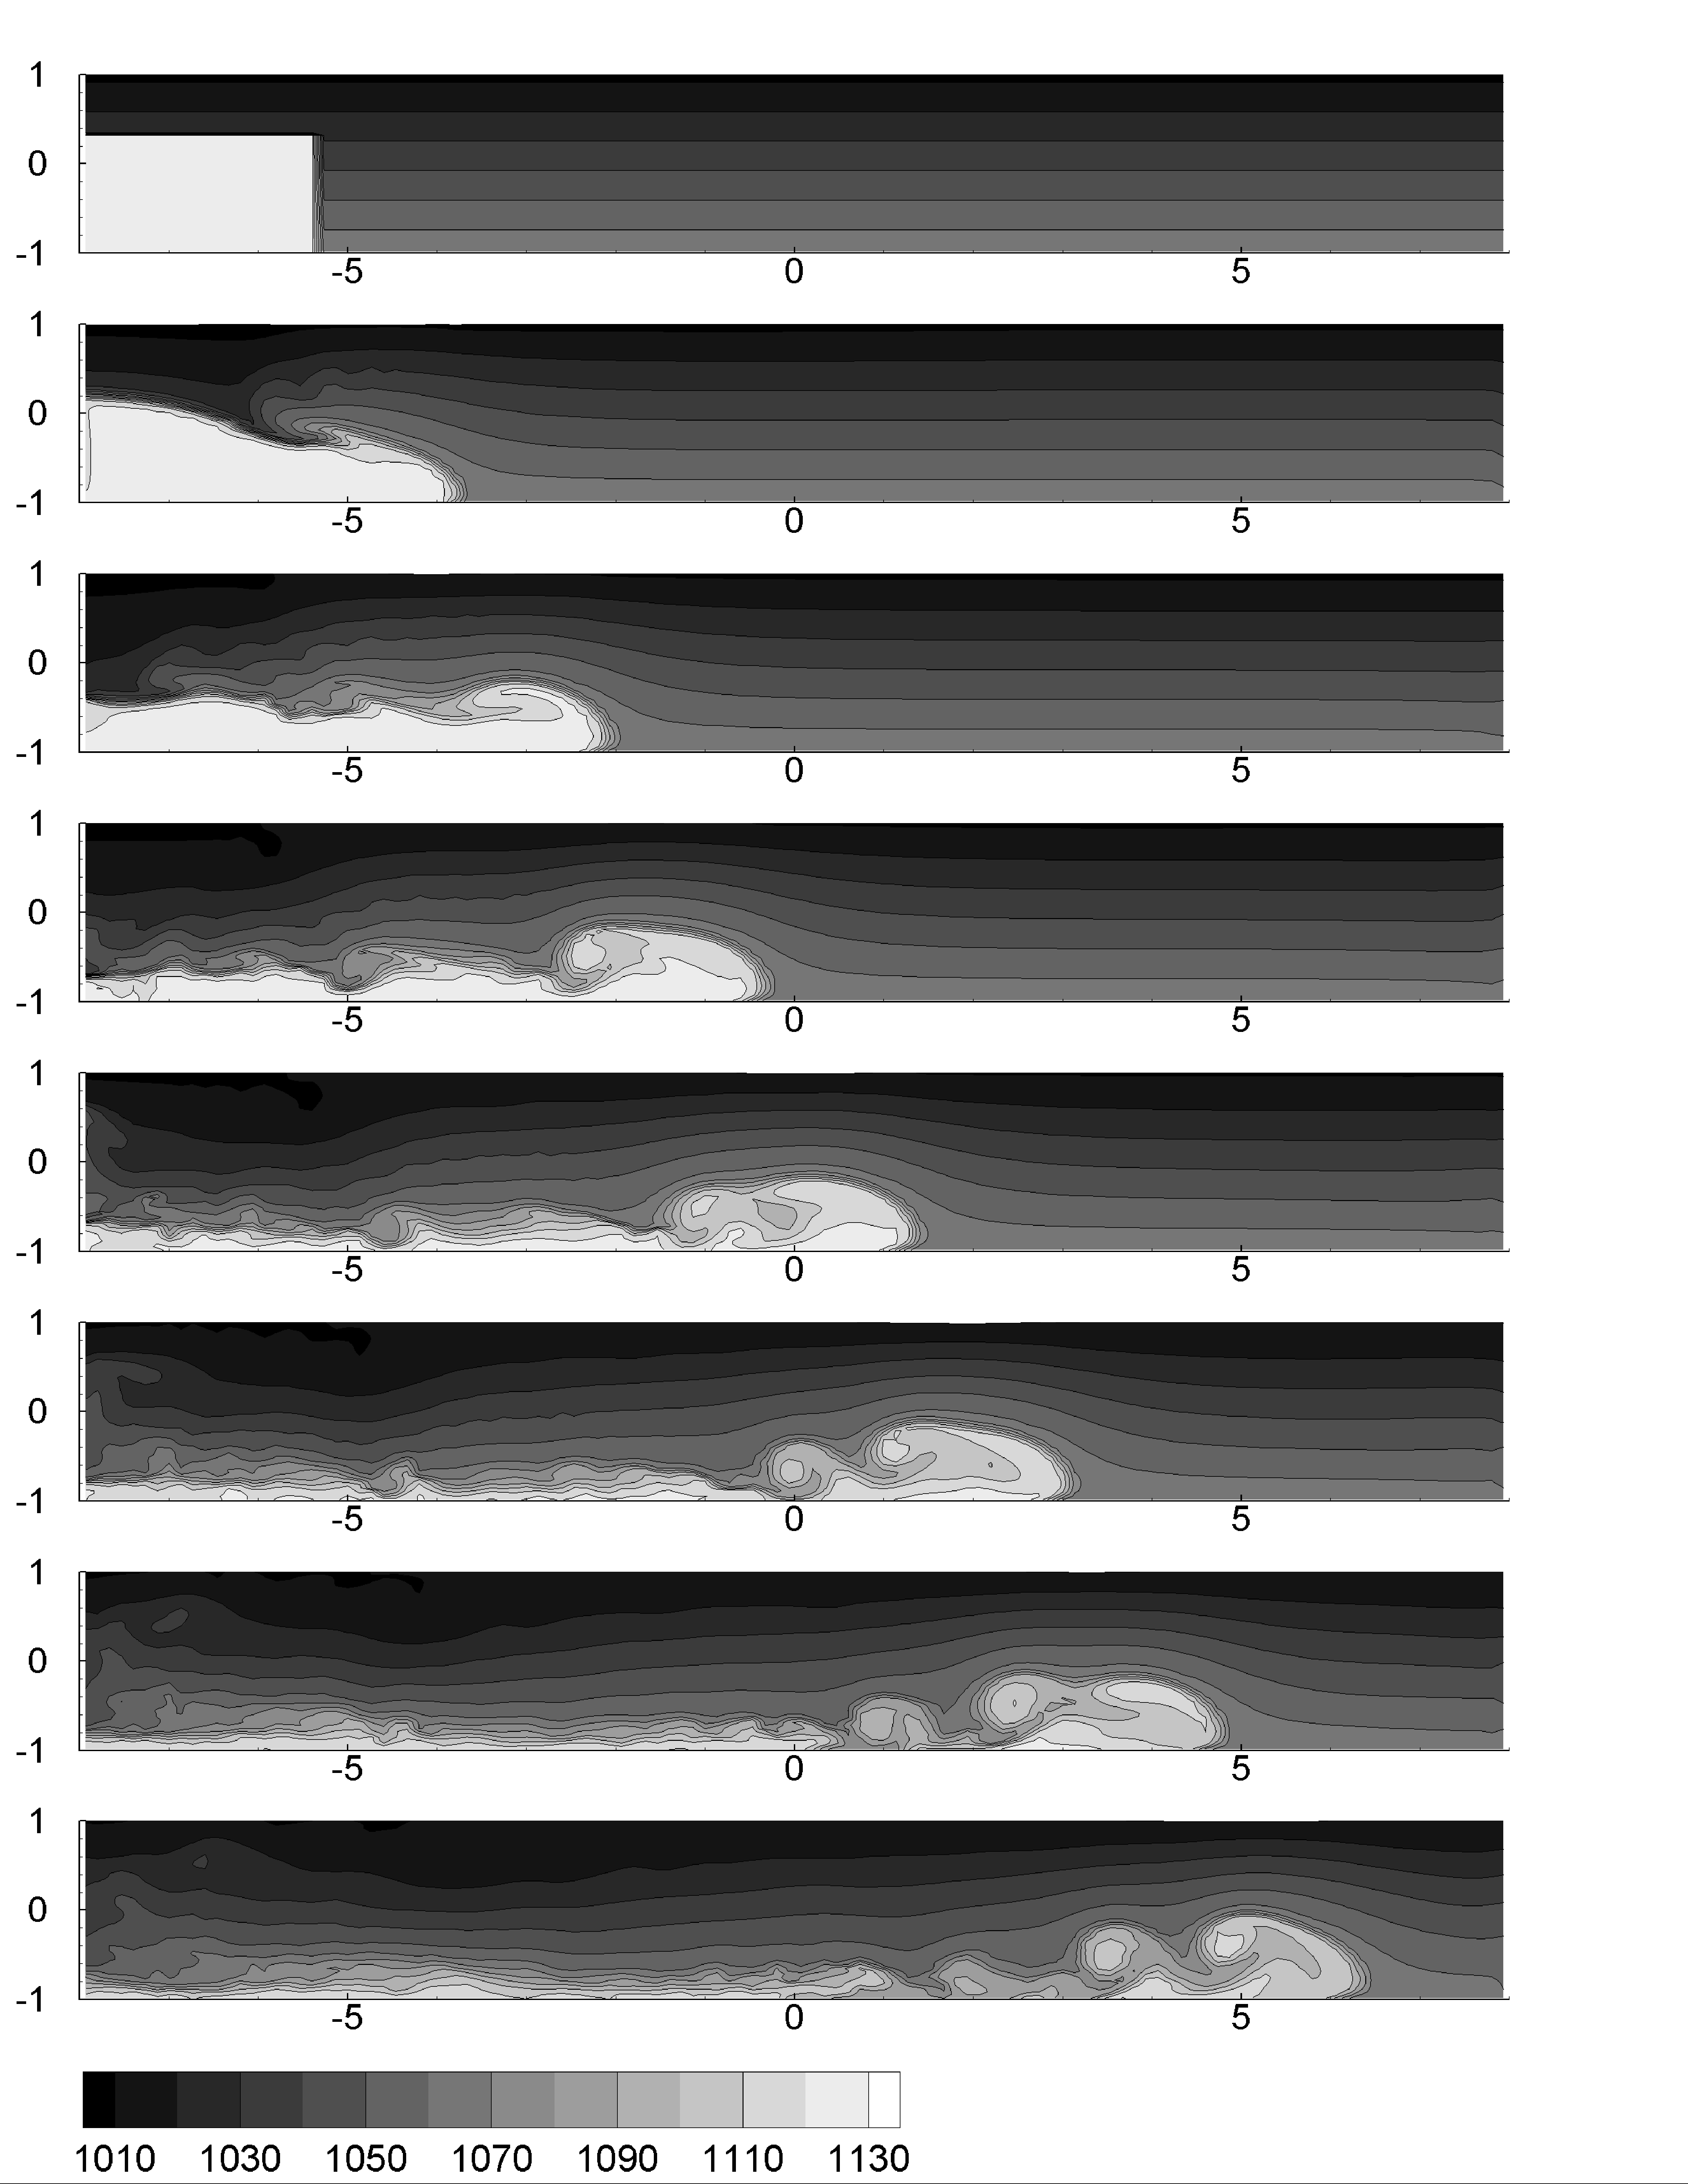
\includegraphics[width=6in]{../figures/GraCur/GraCur-1-Dom-High-RCIP1-Nslip.pdf}
\caption{Numerical simulation of gravity currents with high resolution and non-slip bottom.}
\label{fig:GraCur-1-Dom-High-RCIP1-Nslip}
\end{figure}

\begin{figure}[htbp]
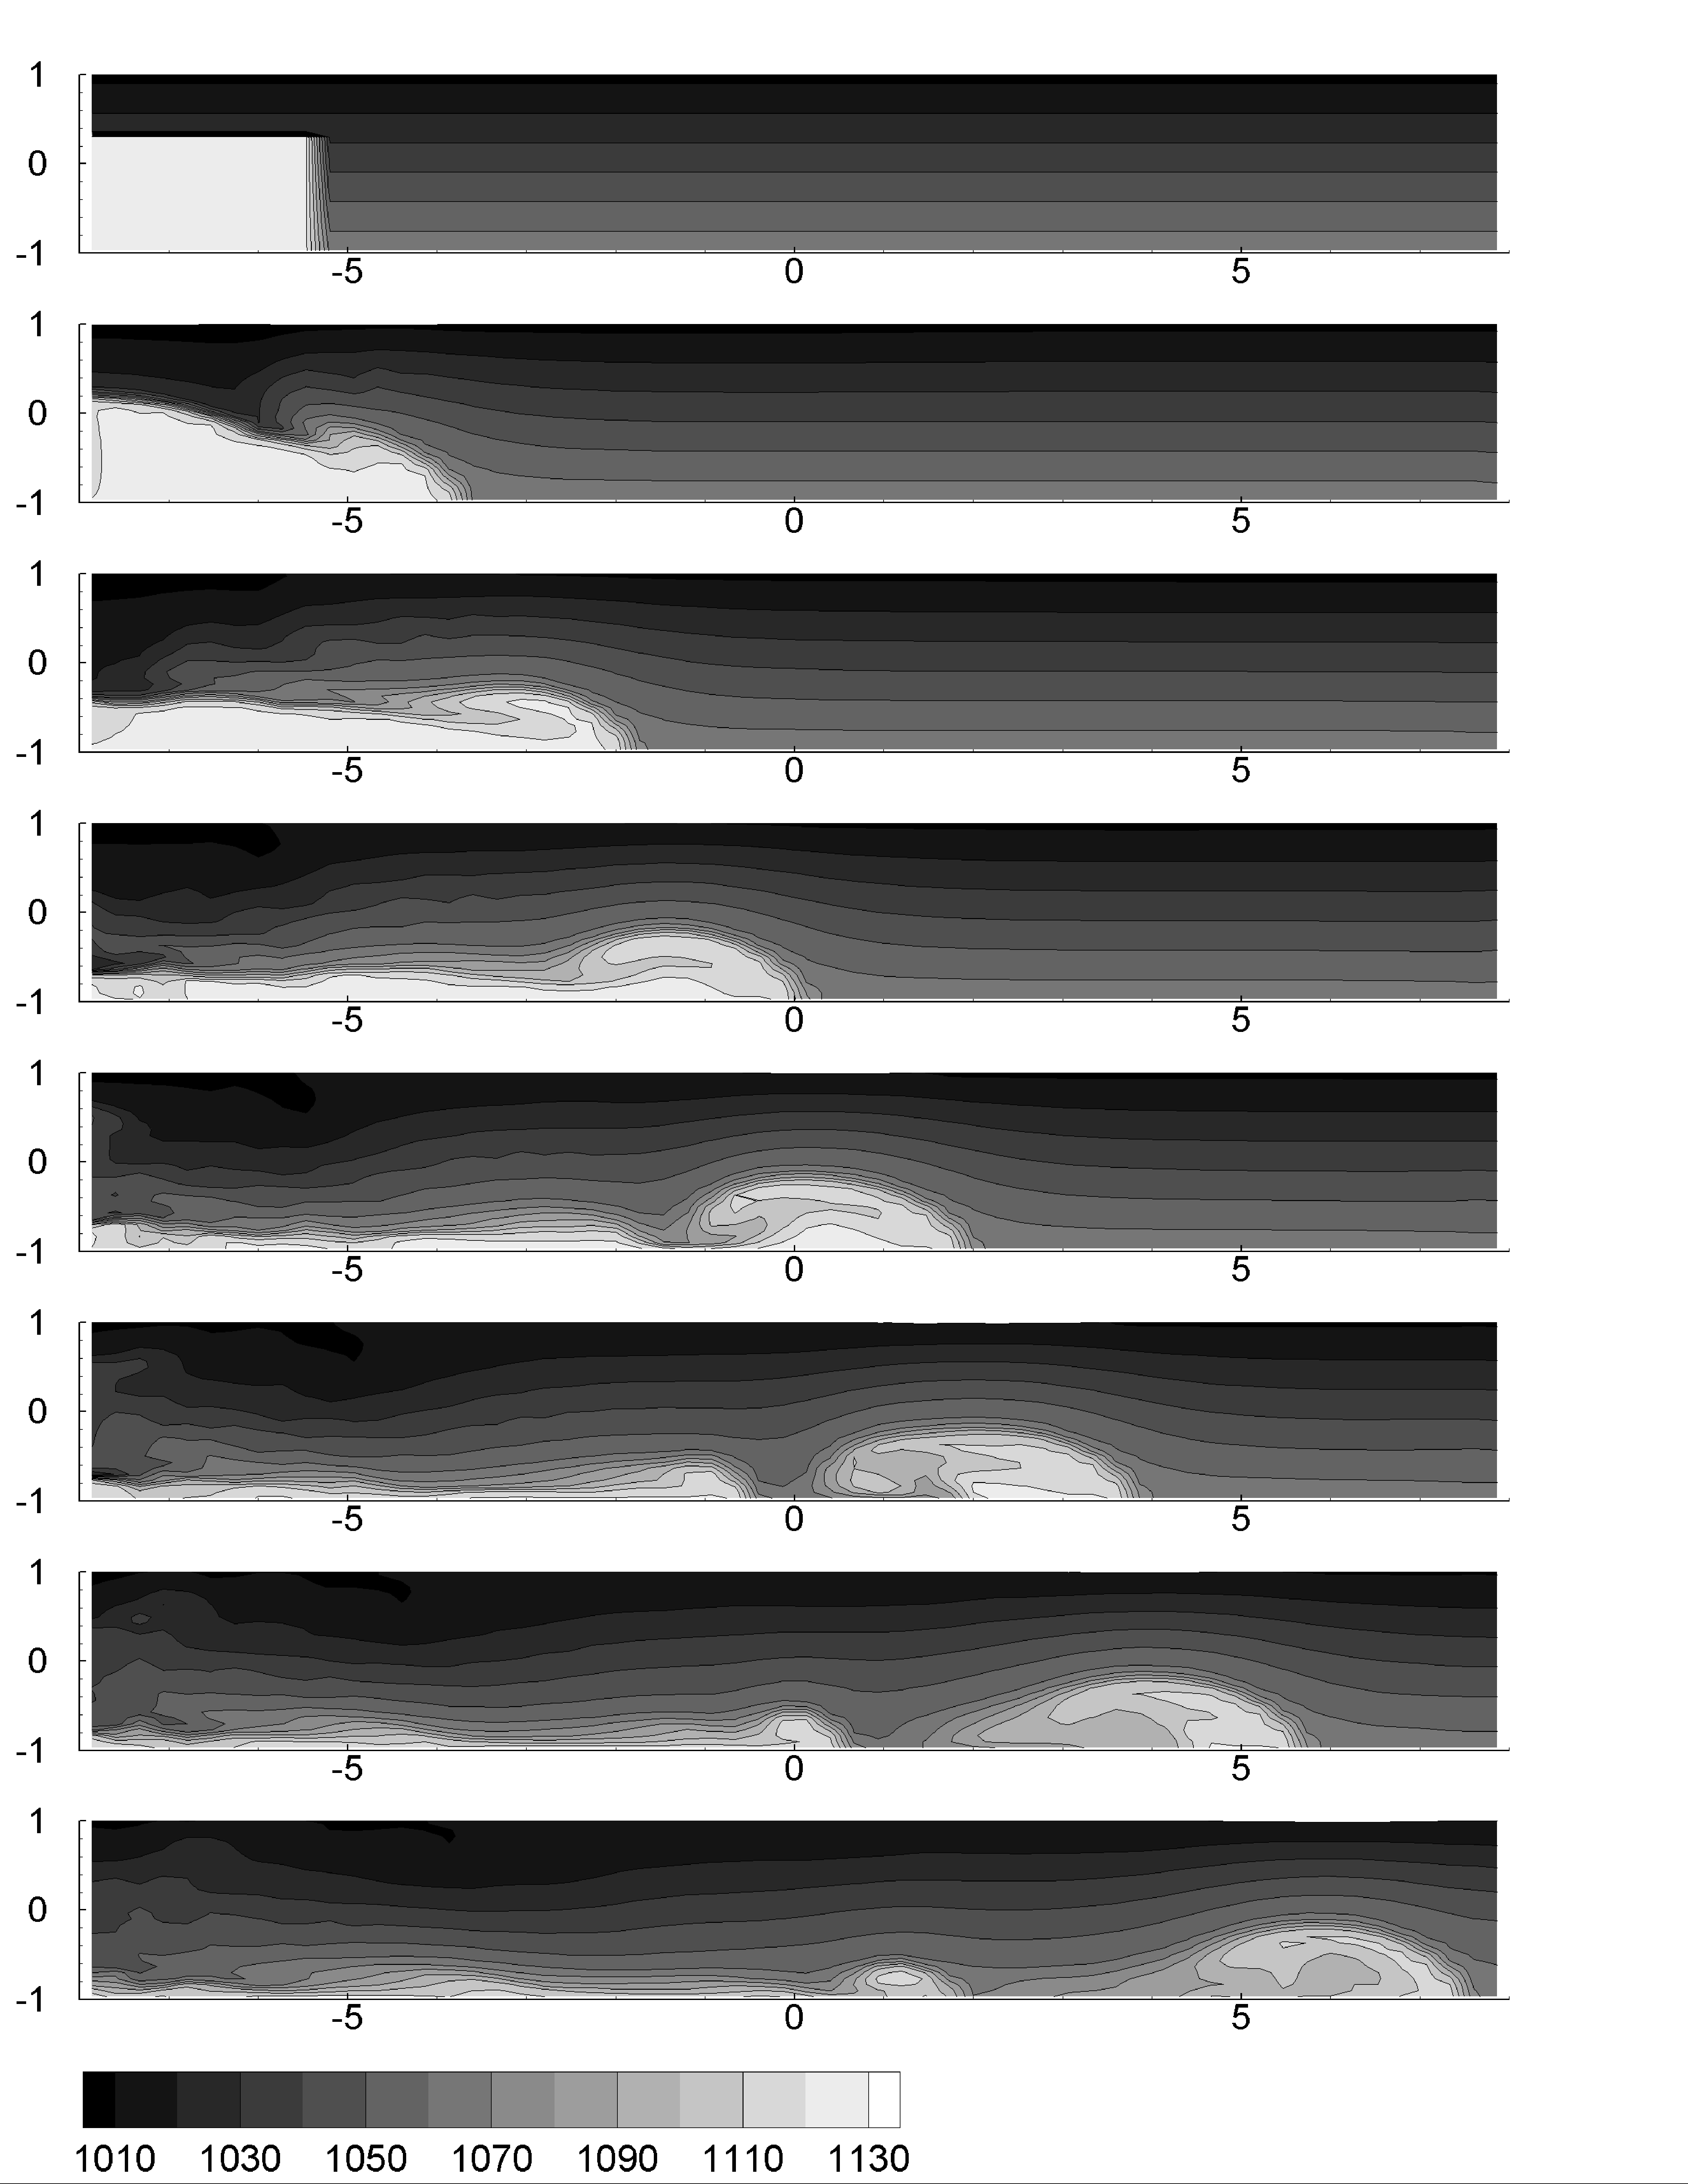
\includegraphics[width=6in]{../figures/GraCur/GraCur-1-Dom-Medium-RCIP1-Slip.pdf}
\caption{Numerical simulation of gravity currents with medium resolution and slip bottom.}
\label{fig:GraCur-1-Dom-Medium-RCIP1-Slip}
\end{figure}

\begin{figure}[htbp]
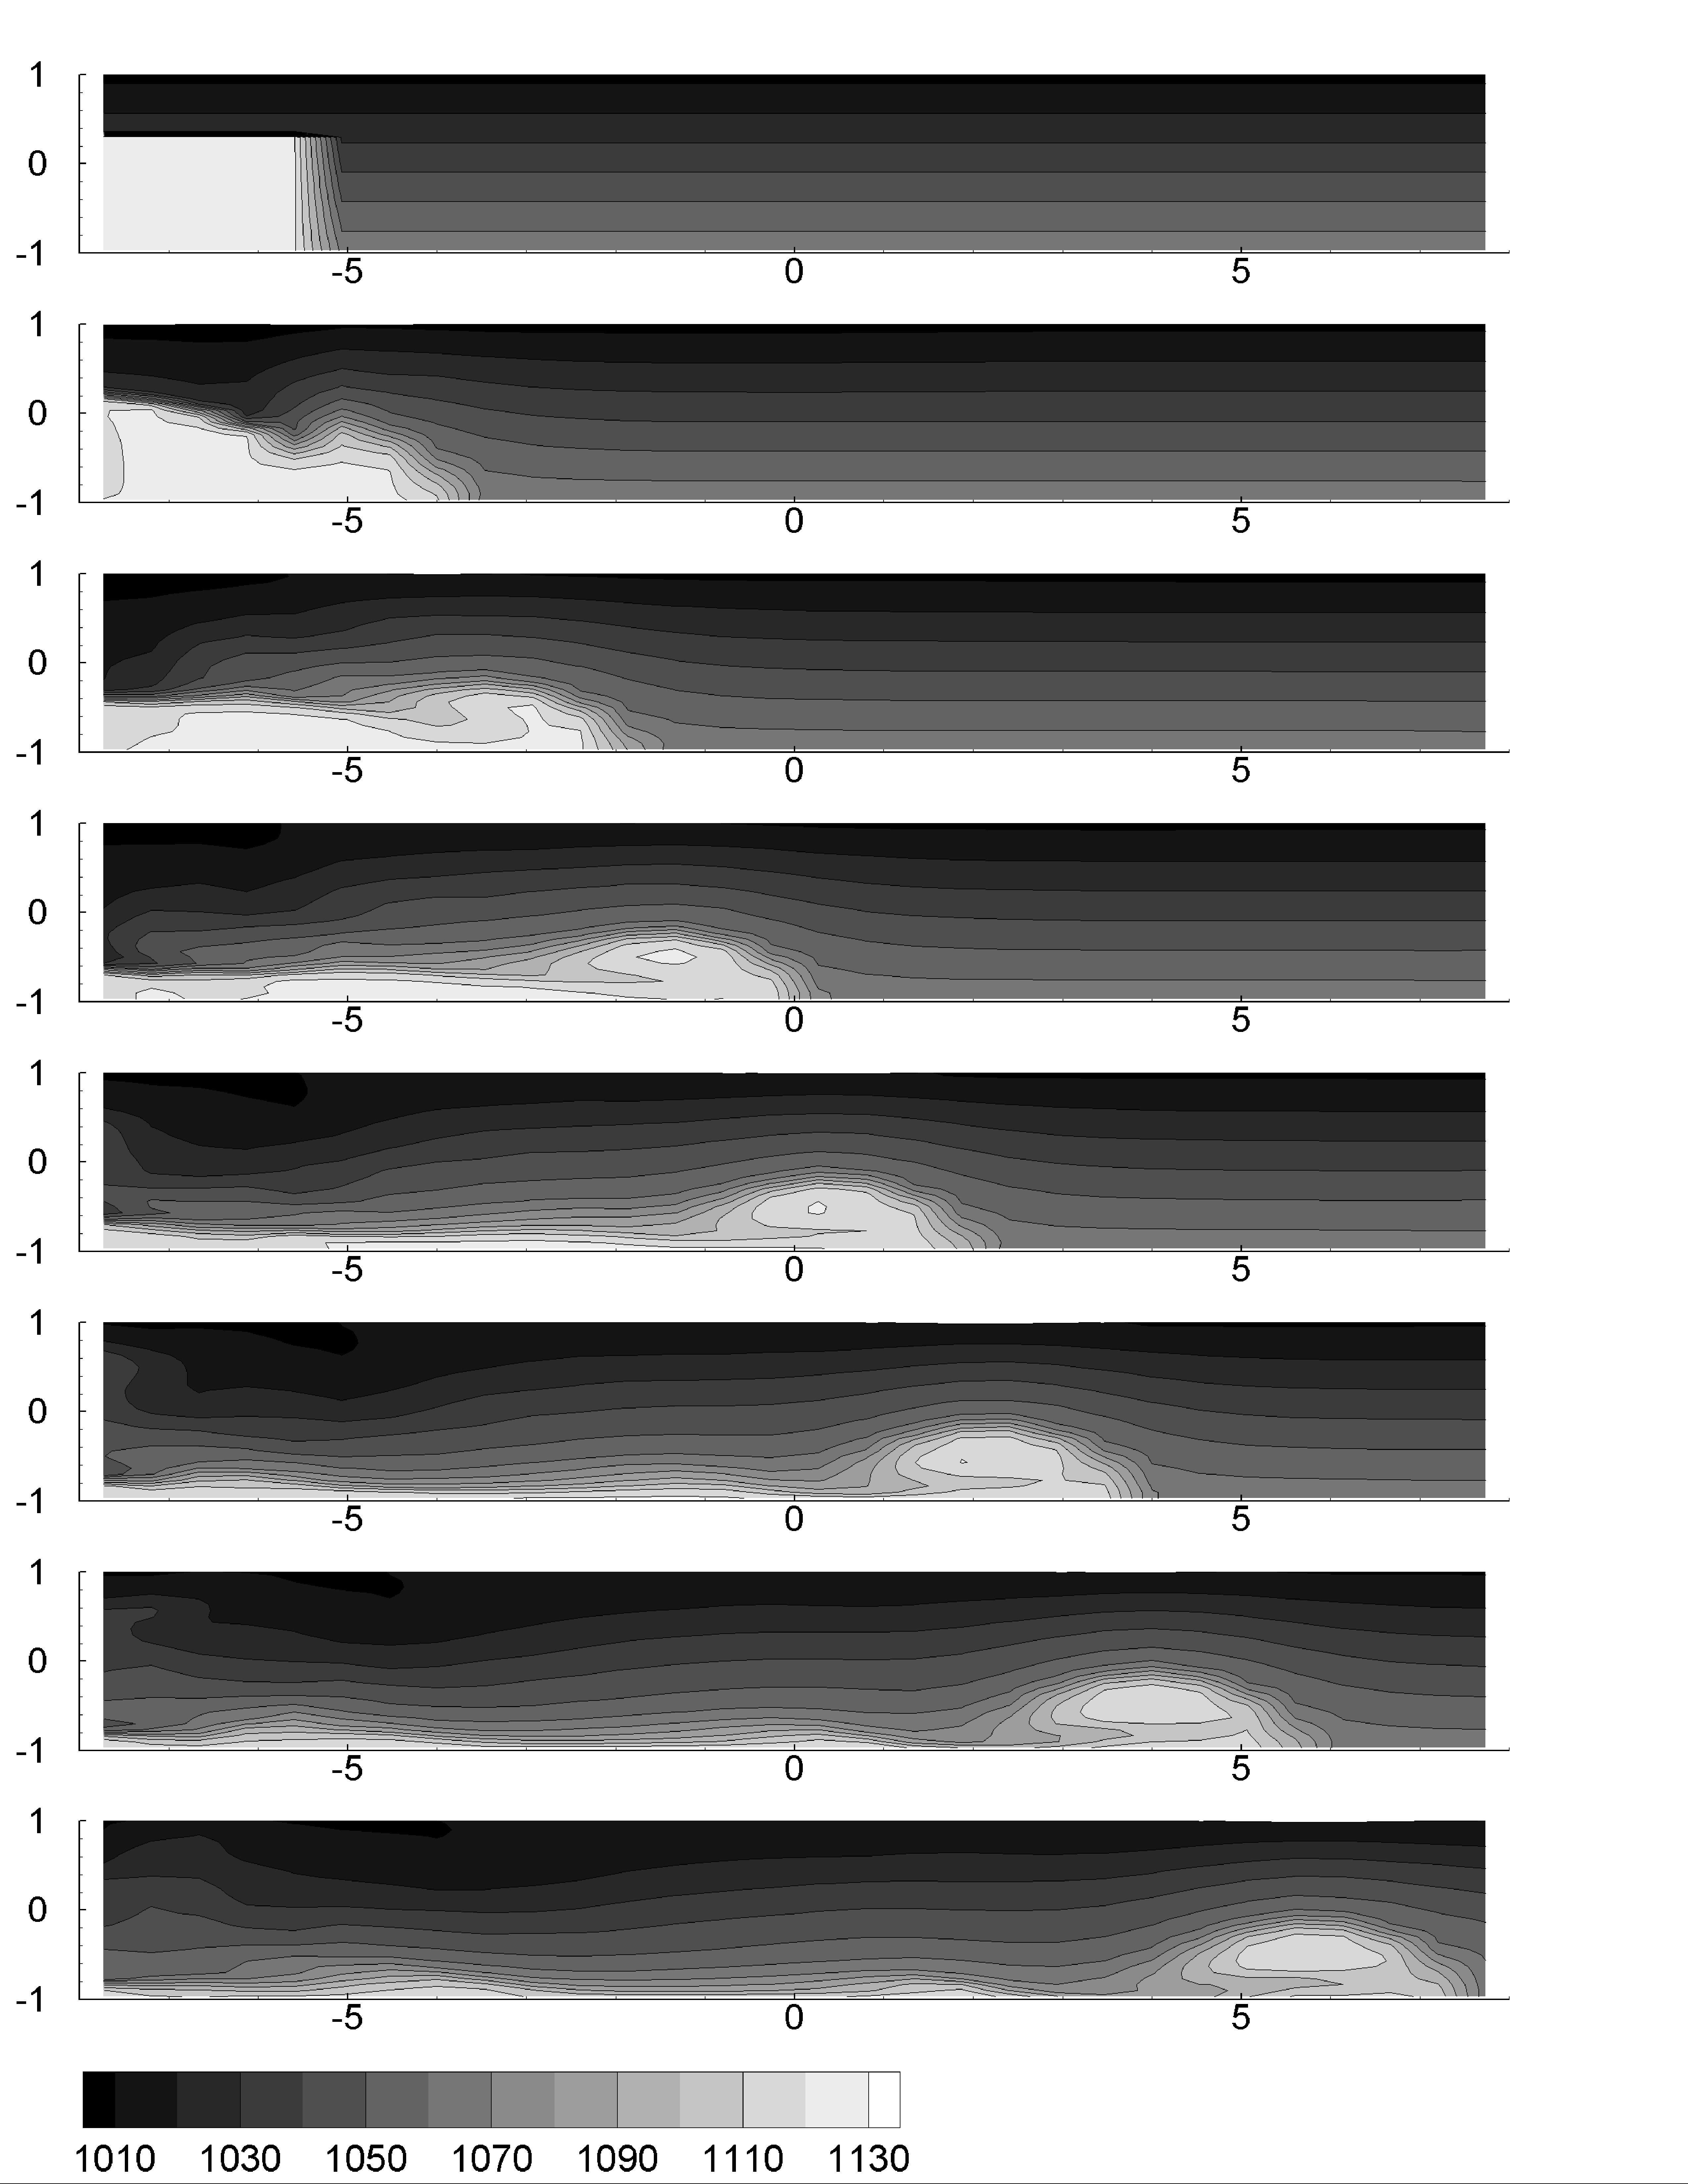
\includegraphics[width=6in]{../figures/GraCur/GraCur-1-Dom-Low-RCIP1-Slip.pdf}
\caption{Numerical simulation of gravity currents with low resolution and slip bottom.}
\label{fig:GraCur-1-Dom-Low-RCIP1-Slip}
\end{figure}

\cp
